\documentclass[a4paper, 14pt]{extreport}

% Схемы
% Качественные характеристики (длинные строки)
% Ссылки

\RequirePackage{cmap}% Для нормальных поиска в тексте и копирования
\RequirePackage[utf8]{inputenc}
\RequirePackage[T2A]{fontenc}
\usepackage[english,russian]{babel}
\usepackage{amssymb,amsfonts,amsmath,mathtext,cite,enumerate,float}
\usepackage{pgfplots}
\usepackage{graphicx}
\usepackage{tocloft}
\usepackage{listings}
\usepackage{caption}
\usepackage{tempora}
\usepackage{setspace}
\usepackage{geometry}
\usepackage{indentfirst}
\usepackage{pdfpages}
\usepackage{enumerate,letltxmacro}
\usepackage{threeparttable}
\usepackage{hyperref}
\usepackage{flafter}
\usepackage{enumitem}
\usepackage{multirow}

\usepackage[figure,table]{totalcount}
\usepackage{lastpage}

\setlist{nosep}

\newcommand{\ssr}[1]{\begin{center}
\LARGE\bfseries{#1}
\end{center} \addcontentsline{toc}{chapter}{#1}  }

\makeatletter
\renewcommand\LARGE{\@setfontsize\LARGE{22pt}{20}}
\renewcommand\Large{\@setfontsize\Large{20pt}{20}}
\renewcommand\large{\@setfontsize\large{16pt}{20}}
\makeatother
\RequirePackage{titlesec}
\titleformat{\chapter}[block]{\hspace{\parindent}\large\bfseries}{\thechapter}{0.5em}{\large\bfseries\raggedright}
\titleformat{name=\chapter,numberless}[block]{\hspace{\parindent}}{}{0pt}{\large\bfseries\centering}
\titleformat{\section}[block]{\hspace{\parindent}\large\bfseries}{\thesection}{0.5em}{\large\bfseries\raggedright}
\titleformat{\subsection}[block]{\hspace{\parindent}\large\bfseries}{\thesubsection}{0.5em}{\large\bfseries\raggedright}
\titleformat{\subsubsection}[block]{\hspace{\parindent}\large\bfseries}{\thesubsection}{0.5em}{\large\bfseries\raggedright}
\titlespacing{\ssr}{12.5mm}{-22pt}{10pt}
\titlespacing{\chapter}{12.5mm}{-22pt}{10pt}
\titlespacing{\section}{12.5mm}{10pt}{10pt}
\titlespacing{\subsection}{12.5mm}{10pt}{10pt}
\titlespacing{\subsubsection}{12.5mm}{10pt}{10pt}

\makeatletter
\renewcommand{\@biblabel}[1]{#1.}
\makeatother
%
%\titleformat{\chapter}[hang]{\LARGE\bfseries}{\hspace{1.25cm}\thechapter}{1ex}{\LARGE\bfseries}
%\titleformat{\section}[hang]{\Large\bfseries}{\hspace{1.25cm}\thesection}{1ex}{\Large\bfseries}
%\titleformat{name=\section,numberless}[hang]{\Large\bfseries}{\hspace{1.25cm}}{0pt}{\Large\bfseries}
%\titleformat{\subsection}[hang]{\large\bfseries}{\hspace{1.25cm}\thesubsection}{1ex}{\large\bfseries}
%\titlespacing{\chapter}{0pt}{-\baselineskip}{\baselineskip}
%\titlespacing*{\section}{0pt}{\baselineskip}{\baselineskip}
%\titlespacing*{\subsection}{0pt}{\baselineskip}{\baselineskip}

\geometry{left=30mm}
\geometry{right=10mm}
\geometry{top=20mm}
\geometry{bottom=20mm}

\onehalfspacing

\renewcommand{\theenumi}{\arabic{enumi}}
\renewcommand{\labelenumi}{\arabic{enumi}\text{)}}
\renewcommand{\theenumii}{.\arabic{enumii}}
\renewcommand{\labelenumii}{\asbuk{enumii}\text{)}}
\renewcommand{\theenumiii}{.\arabic{enumiii}}
\renewcommand{\labelenumiii}{\arabic{enumi}.\arabic{enumii}.\arabic{enumiii}.}

\renewcommand{\cftchapleader}{\cftdotfill{\cftdotsep}}

\addto\captionsrussian{\renewcommand{\figurename}{Рисунок}}
\DeclareCaptionLabelSeparator{dash}{~---~}
\captionsetup{labelsep=dash}

\captionsetup[figure]{justification=centering,labelsep=dash}
\captionsetup[table]{labelsep=dash,justification=raggedright,singlelinecheck=off}

\graphicspath{{images/}}%путь к рисункам

\newcommand{\floor}[1]{\lfloor #1 \rfloor}

\pgfplotsset{width=0.85\linewidth, height=0.5\columnwidth}

\linespread{1.3}

\parindent=1.25cm

%\LetLtxMacro\itemold\item
%\renewcommand{\item}{\itemindent0.75cm\itemold}

\renewcommand{\labelitemi}{---}
\setlist[itemize]{leftmargin=1.25cm, itemindent=0.65cm}
\setlist[enumerate]{leftmargin=1.25cm, itemindent=0.55cm}

\newcommand{\specialcell}[2][c]{%
    \begin{tabular}[#1]{@{}c@{}}#2\end{tabular}}

\frenchspacing

\lstdefinestyle{python}{
    language={Python},
    basicstyle=\footnotesize\ttfamily,
    numbers=none,
    frame=single,
    tabsize=4,
    breaklines=true
}

\begin{document}
    \thispagestyle{empty}

    \noindent \begin{minipage}{0.15\textwidth}
                  
\includegraphics[width=\linewidth]{images/logo}
    \end{minipage}
    \noindent\begin{minipage}{0.85\textwidth}
                 \centering
                 \textbf{Министерство науки и высшего образования Российской Федерации}\\
                 \textbf{Федеральное государственное бюджетное образовательное учреждение высшего образования}\\
                 \textbf{«Московский государственный технический университет имени Н.Э.~Баумана}\\
                 \textbf{(национальный исследовательский университет)»}\\
                 \textbf{(МГТУ им. Н.Э.~Баумана)}
    \end{minipage}

    \noindent\rule{\linewidth}{3pt}
    \newline\newline
    \noindent ФАКУЛЬТЕТ $\underline{\text{«Информатика и системы управления»}}$ \newline\newline
    \noindent КАФЕДРА $\underline{\text{«Программное обеспечение ЭВМ и информационные технологии»}}$

    \vspace{1cm}

    \begin{center}
        \noindent\begin{minipage}{1.3\textwidth}
                     \centering
                     \Large\textbf{  Лабораторная работа № 1}\newline
                     \textbf{по дисциплине <<Анализ алгоритмов>>}\newline\newline
        \end{minipage}
    \end{center}

    \noindent\textbf{Тема} $\underline{\text{Алгоритмы Левенштейна и Дамерау-Левенштейна}}$\newline\newline
    \noindent\textbf{Студент} $\underline{\text{Пантелеев Василий Максимович}}$\newline\newline
    \noindent\textbf{Группа} $\underline{\text{ИУ7-52Б}}$\newline\newline
    \noindent\textbf{Преподаватели} $\underline{\text{Строганов Дмитрий Владимирович}}$\newline

    \begin{center}
        \vfill
        Москва, ~\the\year
    \end{center}

    \clearpage
    \vspace*{-3cm}
    \renewcommand\contentsname{
        \ssr{СОДЕРЖАНИЕ}
    }
    \tableofcontents
    \setcounter{page}{2}


    \clearpage\ssr{ВВЕДЕНИЕ}

    В первой лабораторной работе по анализу алгоритмов рассматривается понятие расстояния Левенштейна.
    Это расстояние определяет минимальное количество операций вставки, удаления и замены, необходимых для преобразования одной строки в другую.
    Расстояние Левенштейна находит широкое применение в различных областях, включая обработку естественного языка, системах автоматического исправления, а также в биоинформатике для сравнения последовательностей.

    Целью данной лабораторной работы является сравнение алгоритмов нахождения расстояния Левенштейна и Дамерау-Левенштейна.
    Для достижения этой цели необходимо решить следующие задачи:

    \begin{itemize}
        \item ознакомиться с теоретическими аспектами расстояния Левенштейна и расстояния Дамерау-Левенштейна;
        \item реализовать рекурсивный алгоритм, рекурсивный алгоритм с мемоизацией, нерекурсивный алгоритм для нахождения расстояния Левенштейна, а также нерекурсивный алгоритм для нахождения расстояния Дамерау-Левенштейна;
        \item сравнить производительность алгоритмов по затраченному процессорному времени и памяти;
        \item обосновать полученные результаты и сделать выводы о характеристиках и применимости каждого алгоритма.
    \end{itemize}

    \clearpage


    \chapter{Аналитическая часть}\label{ch:-4}


    \section{Расстояние Левенштейна}\label{sec:-4}

    Расстояние Левенштейна является мерой различия между двумя строками.
    Оно определяется как минимальное количество односимвольных операций, необходимых для преобразования одной строки в другую.
    Эти операции включают вставку буквы, её удаление и замену буквы на другую.

    Рекуррентная формула расстояния Левенштейна для двух строки $S_{1}$ и $S_{2}$, длинной M и N соответственно:

    \begin{equation}
        \label{eq:L}
        D(i, j) = \begin{cases}
                      0, &\text{i = 0, j = 0}\\
                      i, &\text{j = 0, i > 0}\\
                      j, &\text{i = 0, j > 0}\\
                      min \begin{cases}
                              D(i, j - 1) + 1\\
                              D(i - 1, j) + 1\\
                              D(i - 1, j - 1) + m(S_{1}[i], S_{2}[i]) \\
                      \end{cases}
                      &\text{i > 0, j > 0}
        \end{cases}
    \end{equation}

    \vspace{5mm}

    где функция m определена как:
    \begin{equation}
        \label{eq:m}
        m(a, b) = \begin{cases}
                      0 &\text{если a = b,}\\
                      1 &\text{иначе}
        \end{cases}.
    \end{equation}

    Существует несколько возможных реализаций алгоритма для вычисления расстояния Левенштейна.

    \textbf{Рекурсивный алгоритм.} Это базовая реализация, использующая рекурсию для вычисления расстояния.
    Однако она неэффективна для длинных строк из-за множественных рекурсивных вызовов.

    \textbf{Рекурсивный алгоритм с кэшированием.} Данная реализация использует технику кэширования для хранения результатов уже выполненных подзадач, что снижает количество рекурсивных вызовов и улучшает производительность.

    \textbf{Нерекурсивный алгоритм, основанный на динамическом программировании.} Этот алгоритм использует двумерный массив для хранения промежуточных результатов и заменяет рекурсию итерациями.


    \section{Расстояние Дамерау-Левенштейна}\label{sec:--4}

    Расстояние Дамерау-Левенштейна является расширением расстояния Левенштейна и учитывает дополнительно операцию транспозиции двух соседних символов.
    Расстояние Дамерау-Левенштейна также может быть вычислено с использованием динамического программирования с добавлением дополнительной логики для обработки транспозиции.

    Рекуррентная формула расстояния Дамерау-Левенштейна для двух строки $S_{1}$ и $S_{2}$, длинной M и N соответственно:

    \begin{equation}
        \label{eq:DLev}
        D(i, j) = \begin{cases}
                      i, &\text{j = 0, i > 0} \\
                      j, &\text{i = 0, j > 0} \\
                      D(i - 1, j - 1), &\text{i > 0, j > 0, $S_{1}[i] = S_{2}[j]$} \\
                      1 + \min \begin{cases}
                                   D(i, j - 1)\\
                                   D(i - 1, j)\\
                                   D(i - 1, j - 1) \\
                                   D(i - 2, j - 2) \\
                      \end{cases}, &\begin{aligned}
                                        &\text{$S_{1}[i] = S_{2}[j - 1],$}\\
                                        &\text{$S_{1}[i - 1] = S_{2}[j]$}
                      \end{aligned}\\
                      1 + \min \begin{cases}
                                   D(i, j - 1)\\
                                   D(i - 1, j)\\
                                   D(i - 1, j - 1)\\
                      \end{cases}, &\text{иначе}
        \end{cases}
    \end{equation}

    \section*{Вывод}

    В данном разделе были рассмотрены алгоритмы нахождения расстояния Левенштейна и Дамерау-Левенштейна,
    формулы которых задаются рекуррентно, а следовательно, данные алгоритмы могут быть реализованы рекурсивно и итерационно.
    На вход алгоритмам будут поступать две строки, которые могут содержать как русские, так и английские буквы, также будет предусмотрен ввод пустых строк.

    \clearpage


    \chapter{Конструкторская часть}\label{ch:-3}
    В данном разделе будут приведены схемы алгоритмов нахождения расстояний Левенштейна и Дамерау-Левенштейна.


    \section{Описание алгоритмов}\label{sec:-3}
    На вход алгоритмов подаются 2 строки - str1 и str2, на выходе получается искомое расстояние.

    На схемах~\ref{fig:reklev} ---~\ref{fig:damlev} приведены описания алгоритмов нахождения расстояния Левенштейна и Дамерау-Левенштейна:

    \begin{figure}[H]
        \centering
        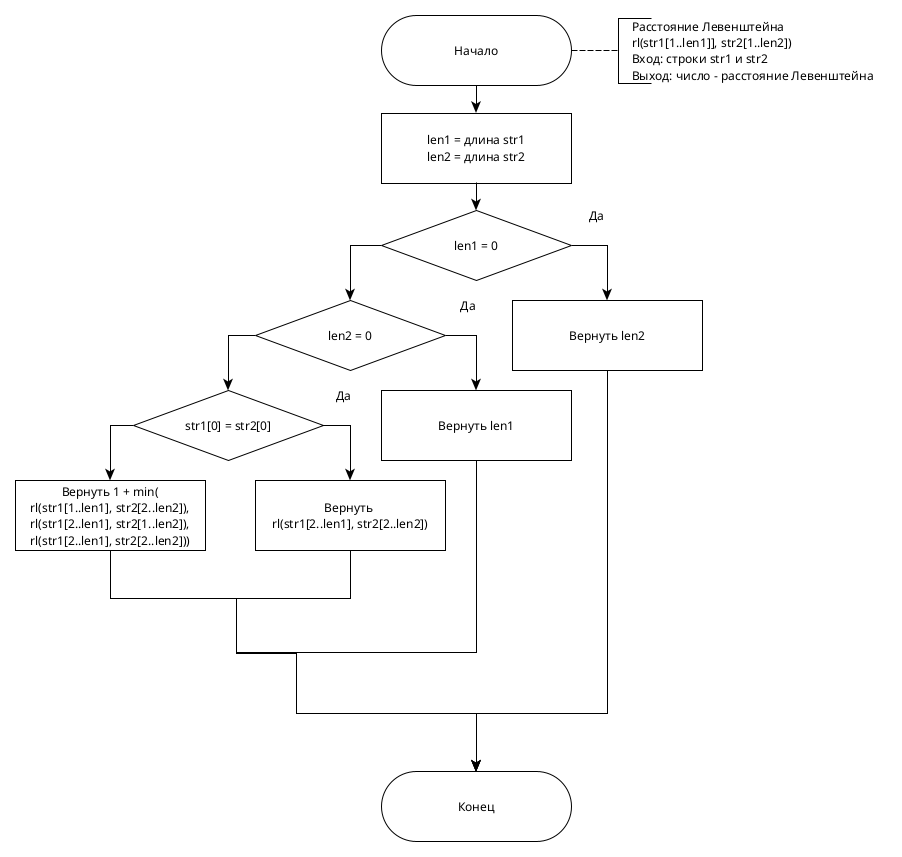
\includegraphics[scale=0.5]{images/s1}
        \caption{Схема рекурсивного алгоритма нахождения расстояния Левенштейна}
        \label{fig:reklev}
    \end{figure}

    \clearpage

    \begin{figure}[H]
        \centering
        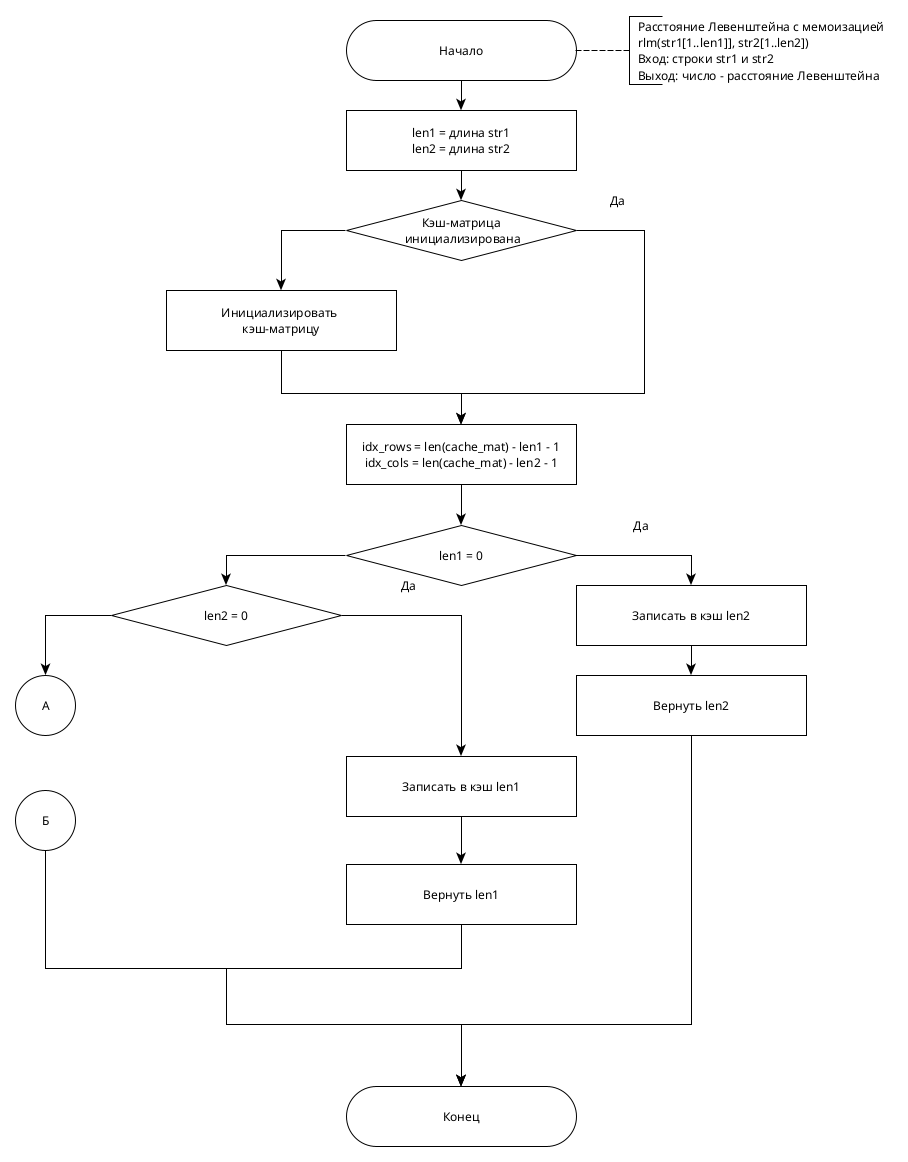
\includegraphics[scale=0.5]{images/s2}
        \caption{Схема рекурсивного алгоритма нахождения расстояния Левенштейна c мемоизацией}
        \label{fig:rekmemlev-1}
    \end{figure}

    \clearpage

    \begin{figure}[H]
        \centering
        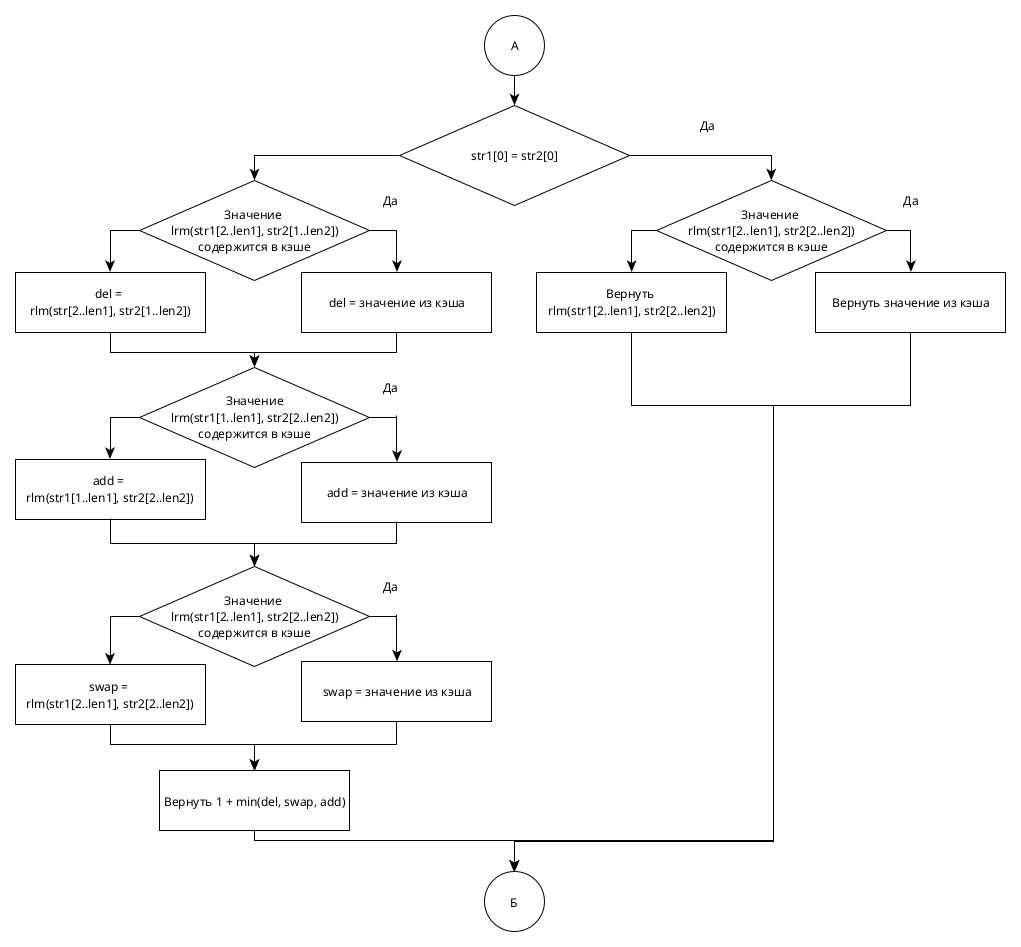
\includegraphics[width=0.95\textwidth, scale=0.45]{images/s3}
        \caption{Схема рекурсивного алгоритма нахождения расстояния Левенштейна c мемоизацией (продолжение)}
        \label{fig:rekmemlev-2}
    \end{figure}

    \clearpage

    \begin{figure}[H]
        \centering
        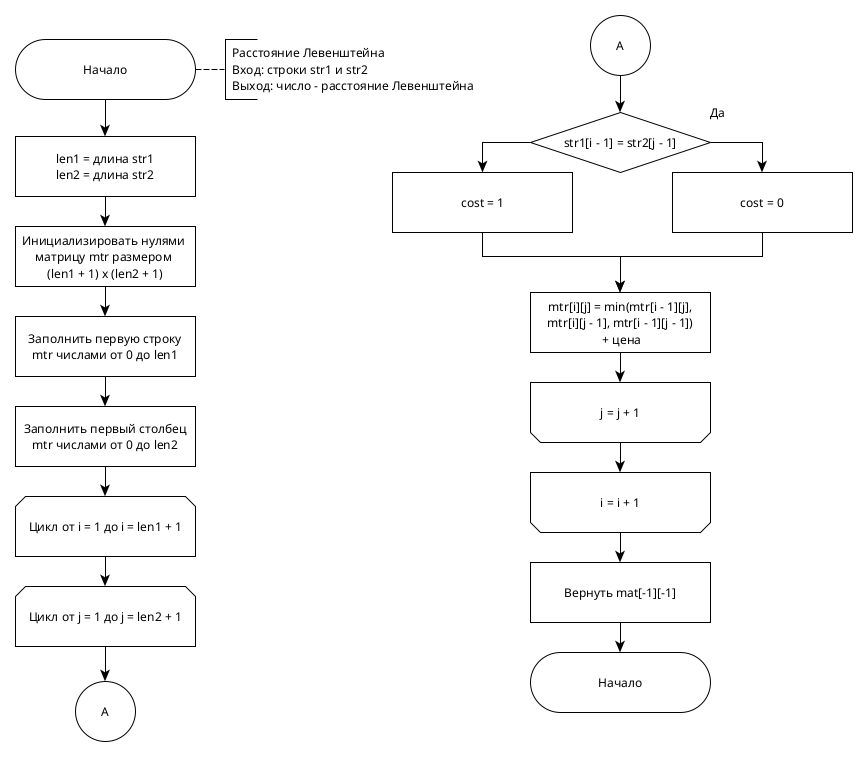
\includegraphics[width=0.95\textwidth, scale=0.6]{images/s4}
        \caption{Схема нерекурсивного алгоритма нахождения расстояния Левенштейна}
        \label{fig:lev}
    \end{figure}

    \clearpage

    \begin{figure}[H]
        \centering
        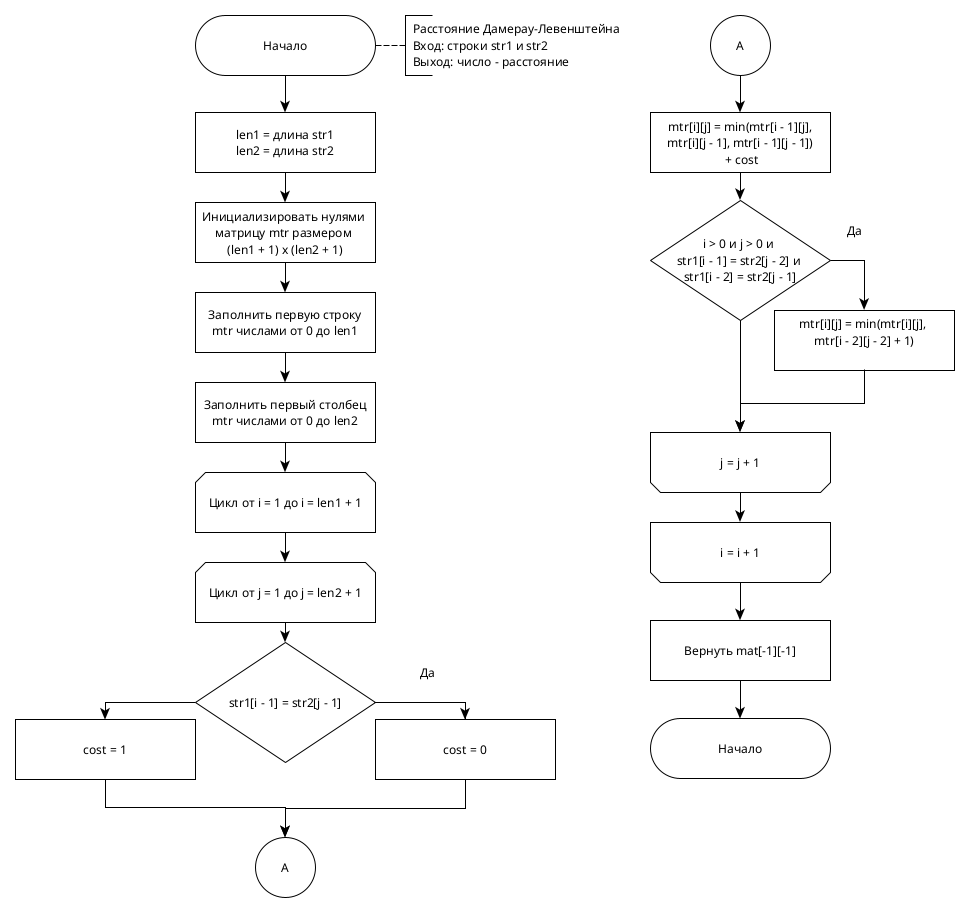
\includegraphics[scale=0.45]{images/s5}
        \caption{Схема нерекурсивного алгоритма нахождения расстояния Дамерау-Левенштейна}
        \label{fig:damlev}
    \end{figure}

    \section*{Вывод}

    В данном разделе на основе теоретических аспектов были разработаны и представлены схемы рекурсивного алгоритма, рекурсивного алгоритма с кэшированием, нерекурсивного алгоритма на основе динамического программирования, а также схема алгоритма Дамерау-Левенштейна.

    \clearpage


    \chapter{Технологическая часть}\label{ch:-2}

    \section{Средства реализации}\label{sec:-2}

    Для реализации алгоритмов в этой лабораторной работы был выбран язык $Python^{[1]}$ по следующим причинам:
    \begin{itemize}
        \item python предоставляет необходимые структуры данных, такие как двумерные списки (массивы);
        \item поддерживаемые библиотеки, такие как matplotlib позволяют визуализировать результаты исследования.
    \end{itemize}


    \section{Реализация алгоритмов}\label{sec:--3}

    В листингах~\ref{lst:reklev} ---~\ref{lst:damlev} представлены реализации алгоритмов.

    \begin{lstlisting}[style=python, caption=Рекурсивный алгоритм Левенштейна,label={lst:reklev}]
def levenshtein_recursive(str1, str2):
len1 = len(str1)
len2 = len(str2)

if len1 == 0:
return len2
elif len2 == 0:
return len1
elif str1[0] == str2[0]:
return levenshtein_recursive(str1[1:], str2[1:])

return 1 + min(
levenshtein_recursive(str1[1:], str2),
levenshtein_recursive(str1, str2[1:]),
levenshtein_recursive(str1[1:], str2[1:])
)
    \end{lstlisting}

    \begin{lstlisting}[style=python, caption=Рекурсивный алгоритм Левенштейна с Мемоизацией,label={lst:rekmemlev}]
def levenshtein_recursive_memo(str1, str2, cache_matrix=None):
len1 = len(str1)
len2 = len(str2)

if cache_matrix is None:
cache_matrix = [[-1] * (len2 + 1) for _ in range(len1 + 1)]

idx_rows = len(cache_matrix) - len1 - 1
idx_cols = len(cache_matrix[0]) - len2 - 1

if len1 == 0:
cache_matrix[idx_rows][idx_cols] = len2
return len2
elif len2 == 0:
cache_matrix[idx_rows][idx_cols] = len1
return len1
elif str1[0] == str2[0]:
curr = cache_matrix[idx_rows + 1][idx_cols + 1]
return curr if curr != -1 else levenshtein_recursive_memo(str1[1:], str2[1:], cache_matrix)

delete = cache_matrix[idx_rows + 1][idx_cols]
add = cache_matrix[idx_rows][idx_cols + 1]
swap = cache_matrix[idx_rows + 1][idx_cols + 1]

return 1 + min(
delete if delete != -1 else levenshtein_recursive_memo(str1[1:], str2, cache_matrix),
add if add != -1 else levenshtein_recursive_memo(str1, str2[1:], cache_matrix),
swap if swap != -1 else levenshtein_recursive_memo(str1[1:], str2[1:], cache_matrix)
)
    \end{lstlisting}

    \begin{lstlisting}[style=python, caption=Нерекурсивный алгоритм Левенштейна,label={lst:lev}]
def levenshtein(str1, str2):
len1 = len(str1)
len2 = len(str2)

cache_matrix = [[0] * (len2 + 1) for _ in range(len1 + 1)]

for i in range(len1 + 1):
cache_matrix[i][0] = i
for j in range(len2 + 1):
cache_matrix[0][j] = j

for i in range(1, len1 + 1):
for j in range(1, len2 + 1):
cost = 0 if str1[i - 1] == str2[j - 1] else 1

cache_matrix[i][j] = min(
cache_matrix[i - 1][j],
cache_matrix[i][j - 1],
cache_matrix[i - 1][j - 1]
) + cost

return cache_matrix[-1][-1]
    \end{lstlisting}

    \begin{lstlisting}[style=python, caption=Нерекурсивный алгоритм Дамерау-Левенштейна,label={lst:damlev}]
def damerau_levenshtein(str1, str2):
len1 = len(str1)
len2 = len(str2)

cache_matrix = [[0] * (len2 + 1) for _ in range(len1 + 1)]

for i in range(len1 + 1):
cache_matrix[i][0] = i
for j in range(len2 + 1):
cache_matrix[0][j] = j

for i in range(1, len1 + 1):
for j in range(1, len2 + 1):
cost = 0 if str1[i - 1] == str2[j - 1] else 1

cache_matrix[i][j] = min(
cache_matrix[i - 1][j],
cache_matrix[i][j - 1],
cache_matrix[i - 1][j - 1]
) + cost

if i > 1 and j > 1 and str1[i - 1] == str2[j - 2] and str1[i - 2] == str2[j - 1]:
cache_matrix[i][j] = min(cache_matrix[i][j], cache_matrix[i - 2][j - 2] + 1)

return cache_matrix[-1][-1]
    \end{lstlisting}

    \clearpage


    \section{Функциональные тесты}\label{sec:-}

    В таблице~\ref{tbl:func_test} представлены функциональные тесты для проверки корректности работы программы.

    \begin{table}[h]
        \begin{center}
            \caption{\label{tbl:func_test} Функциональные тесты}
            \begin{tabular}{|c|c|c|c|}
                \hline
                $str_{1}$ & $str_{2}$ & Левенштейн & Дамерау-Левенштейн
                \\ \hline
                «» & «» & 0 & 0
                \\ \hline
                abc & «» & 3 & 3
                \\ \hline
                «» & abc & 3 & 3
                \\ \hline
                abc & abc & 0 & 0
                \\ \hline
                abc & xyz & 3 & 3
                \\ \hline
                abc & abcd & 1 & 1
                \\ \hline
                abcd & abc & 1 & 1
                \\ \hline
                kitten & sitting & 3 & 3
                \\ \hline
                reka & muka & 2 & 2
                \\ \hline
                apple & appel & 2 & 1
                \\ \hline
            \end{tabular}
        \end{center}
    \end{table}

    \section*{Вывод}

    В технологической части были представлены листинги реализованных алгоритмов, включая рекурсивные и нерекурсивные версии нахождения расстояния Левенштейна и Дамерау-Левенштейна.
    Также были проведены функциональные тесты, которые подтвердили корректность работы всех алгоритмов на различных входных данных, включая граничные случаи.
    Результаты тестов показали, что разработанные реализации соответствуют поставленным требованиям.

    \clearpage


    \chapter{Исследовательская часть}\label{ch:-}


    \section{Технические характеристики ЭВМ}\label{sec:--2}
    Все замеры проводились на ЭВМ, характеристики которой приведены ниже:
    \begin{itemize}
        \item процессор: AMD Ryzen™ 7--5800H with Radeon™ Graphics × 16;
        \item ОС: 64-разрядная операционная система Ubuntu 24.04.1 LTS;
        \item оперативная память: 16,0 ГБ.
    \end{itemize}


    \section{Сравнение по времени}

    Время выполнения работы алгоритмов представлено в секундах.
    Для повышения точности измерений проводилось 200 замеров.
    Замеры проводились использованием функции $process\_time^{[2]}$ модуля time стандартной библиотеки Python, позволяющей измерять процессорное время, потраченное на выполнение алгоритма.
    Графики построены при помощи средств библиотеки $matplotlib^{[3]}$.

    В таблице~\ref{tbl:time_cmp} приведено сравнение алгоритмов по времени выполнения на размерах строк от 1 до 10 с шагом 1.
    На графике~\ref{fig:cmp} приведена визуализация результатов.


    \begin{table}[H]
        \begin{center}
            \caption{\label{tbl:time_cmp} Сравнение алгоритмов по времени выполнения}
            \begin{tabular}{|c|r|r|r|r|}
                \hline
                Размер строк & Рекурсивный & C кэшем & Нерекурсивный & Дамерау
                \\ \hline
                1 & $1 \times 10^{-6}$ & $2 \times 10^{-6}$ & $1 \times 10^{-6}$ & $2 \times 10^{-6}$
                \\ \hline
                2 & $3 \times 10^{-6}$ & $4 \times 10^{-6}$ & $2 \times 10^{-6}$ & $3 \times 10^{-6}$
                \\ \hline
                3 & $1 \times 10^{-5}$ & $1 \times 10^{-5}$ & $4 \times 10^{-6}$ & $4 \times 10^{-6}$
                \\ \hline
                4 & $5 \times 10^{-5}$ & $5 \times 10^{-5}$ & $5 \times 10^{-6}$ & $6 \times 10^{-6}$
                \\ \hline
                5 & $3 \times 10^{-4}$ & $2 \times 10^{-4}$ & $7 \times 10^{-6}$ & $9 \times 10^{-6}$
                \\ \hline
                6 & $1 \times 10^{-3}$ & $9 \times 10^{-4}$ & $9 \times 10^{-6}$ & $1.2 \times 10^{-5}$
                \\ \hline
                7 & $7 \times 10^{-3}$ & $6 \times 10^{-3}$ & $1.3 \times 10^{-5}$ & $1.5 \times 10^{-5}$
                \\ \hline
                8 & 0.04 & 0.03 & $1.6 \times 10^{-5}$ & $2.0 \times 10^{-5}$
                \\ \hline
                9 & 0.20 & 0.16 & $2.0 \times 10^{-5}$ & $2.4 \times 10^{-5}$
                \\ \hline
                10 & 1.00 & 0.88 & $2.4 \times 10^{-5}$ & $3.0 \times 10^{-5}$
                \\ \hline
            \end{tabular}
        \end{center}
    \end{table}

    \begin{figure}[H]
        \centering
        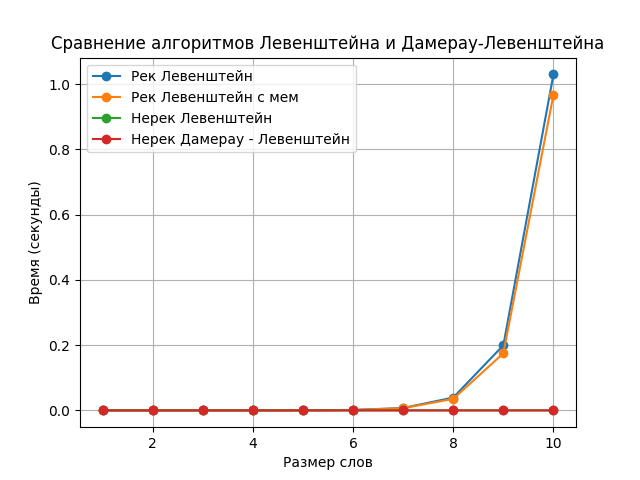
\includegraphics[scale=1]{images/graph1}
        \caption{Сравнение алгоритмов по времени выполнения}
        \label{fig:cmp}
    \end{figure}

    В таблице~\ref{tbl:not_rec_time_cmp} приведено сравнение нерекурсивных алгоритмов по времени выполнения на размерах строк от 10 до 500.
    На графике~\ref{fig:notrek_cmp} приведена визуализация результатов.

    \begin{table}[H]
        \begin{center}10
            \caption{\label{tbl:not_rec_time_cmp} Сравнение нерекурсивных алгоритмов по времени выполнения}
            \begin{tabular}{|c|r|r|}
                \hline
                Размер строк & Левенштейн & Дамерау-Левенштейн
                \\ \hline
                10 & $2.4 \times 10^{-5}$ & $3.0 \times 10^{-5}$
                \\ \hline
                20 & $9.3 \times 10^{-5}$ & $1.1 \times 10^{-4}$
                \\ \hline
                30 & $3.7 \times 10^{-4}$ & $4.5 \times 10^{-4}$
                \\ \hline
                50 & $5.8 \times 10^{-4}$ & $7.2 \times 10^{-4}$
                \\ \hline
                100 & $2.2 \times 10^{-3}$ & $2.8 \times 10^{-3}$
                \\ \hline
                150 & $4.9 \times 10^{-3}$ & $6.3 \times 10^{-3}$
                \\ \hline
                200 & $8.7 \times 10^{-3}$ & 0.01
                \\ \hline
                300 & 0.02 & 0.03
                \\ \hline
                400 & 0.04 & 0.05
                \\ \hline
                500 & 0.06 & 0.08
                \\ \hline
            \end{tabular}
        \end{center}
    \end{table}

    \clearpage\begin{figure}[H]
                  \centering
                  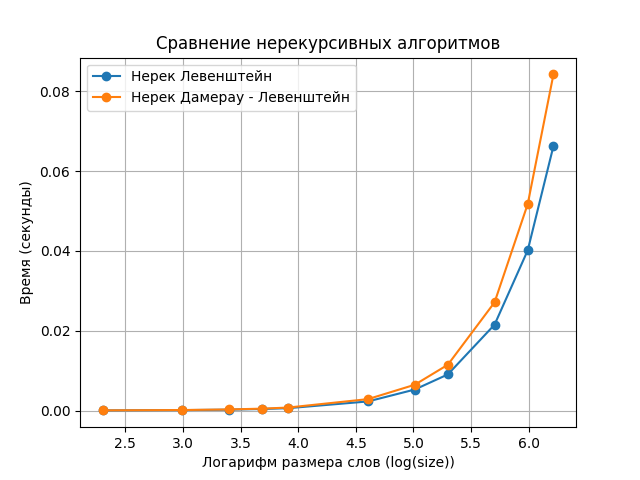
\includegraphics[scale=0.7]{images/graph2}
                  \caption{Сравнение нерекурсивных алгоритмов по времени выполнения}
                  \label{fig:notrek_cmp}
    \end{figure}


    \section{Сравнение по памяти}\label{sec:--}
    В таблице~\ref{tbl:mem_comp} приведено сравнение различных реализаций по памяти.
    Нерекурсивные алгоритмы
    Левенштейна и Дамерау-Левенштейна эквивалентны по расходу памяти.

    Затраты памяти для алгоритмов:
    \begin{itemize}
        \item рекурсивный алгоритм нахождения расстояния Левенштейна -- len1 + len2;
        \item рекурсивный алгоритм нахождения расстояния Левенштейна с мемоизацией -- len1 * len2 + len1 + len2;
        \item нерекурсивный алгоритм нахождения расстояния Левенштейна -- len1 * len2 + len1 + len2;
        \item нерекурсивный алгоритм нахождения расстояния Дамерау-Левенштейна -- len1 * len2 + len1 + len2.
    \end{itemize}

    len1 и len2 - длины строк на входе.

    \clearpage\begin{table}[H]
                  \begin{center}
                      \caption{\label{tbl:mem_comp} Сравнение по памяти двух строк длины len1 и len2 соответственно}
                      \begin{tabular}{|c|c|r|r|r|}
                          \hline
                          len1 & len2 & Рекурсивно, байт & Рекурсивно + мем, байт & Нерекурсивно, байт
                          \\ \hline
                          1 & 1 & 20 & 26 & 10
                          \\ \hline
                          10 & 10 & 20 & 161 & 145
                          \\ \hline
                          100 & 100 & 200 & 10421 & 10405
                          \\ \hline
                          1000 & 1000 & 2000 & 1004021 & 1004005
                          \\ \hline
                      \end{tabular}
                  \end{center}
    \end{table}

    \section*{Вывод}

    В исследовательской части было проведено сравнение различных реализаций алгоритмов нахождения расстояния Левенштейна и Дамерау-Левенштейна по времени выполнения и потребляемым ресурсам.
    Анализ показал, что рекурсивный алгоритм с кэшированием выигрывает по времени примерно в 1.25 раза по сравнению с базовым рекурсивным подходом за счет уменьшения числа повторных вычислений.
    Однако этот алгоритм требует большего объема памяти, так как хранит промежуточные результаты для всех подзадач.

    Рекурсивные алгоритмы имеют высокую временную сложность, но на строках, размером до 6, разница не существенна.
    В свою очередь, нерекурсивные алгоритмы, основанные на динамическом программировании, демонстрируют лучшую производительность на длинных словах (от 6 символов) за счет более эффективного использования памяти и отсутствия накладных расходов, связанных с рекурсией.

    \clearpage

    \ssr{ЗАКЛЮЧЕНИЕ}

    В ходе работы было установлено, что существует различие в временной эффективности между рекурсивными и нерекурсивными реализациями алгоритмов Левенштейна и Дамерау-Левенштейна. Разработанное программное обеспечение позволило осуществить замеры процессорного времени выполнения для различных длин строк, что подтвердило теоретические ожидания.

    Результаты исследования показали, что нерекурсивная матричная реализация алгоритмов превосходит рекурсивные подходы по времени выполнения, особенно при увеличении длины обрабатываемых строк (от 6 символов). Однако следует отметить, что данная матричная реализация требует больше памяти, что может быть критично в условиях ограниченных ресурсов.

    Оптимизация рекурсивного алгоритма выигрывает у обычной реализации по времени (в 1.25 раза), но проигрывает по памяти из-за необходимости хранить кэш-матрицу.

    Таким образом, выбор между рекурсивной и нерекурсивной реализацией данных алгоритмов зависит от конкретных требований к производительности и ресурсам.


    В ходе выполненной работы были выполнены следующие задачи:
    \begin{itemize}
        \item реализованы различные алгоритмы для вычисления расстояния Левенштейна и Дамерау-Левенштейна;
        \item проведено сравнение алгоритмов по времени выполнения и памяти;
        \item полученные результаты обоснованы.
    \end{itemize}

%    В ходе выполненной работы были реализованы различные алгоритмы для вычисления расстояния Левенштейна и Дамерау-Левенштейна, включая рекурсивные и нерекурсивные подходы.
%    Проведенные исследования показали, что каждый из методов имеет свои преимущества и недостатки в зависимости от требований к времени выполнения и использованию памяти.
%    Результаты работы подтвердили корректность всех реализаций и позволили оценить их эффективность.

    \clearpage

    \renewcommand{\bibname}{\begin{center}
                                \Large СПИСОК ИСПОЛЬЗОВАННЫХ ИСТОЧНИКОВ
    \end{center}}
    \addcontentsline{toc}{chapter}{СПИСОК ИСПОЛЬЗОВАННЫХ ИСТОЧНИКОВ}
    \begin{thebibliography}{}
        \bibitem{bi1}
        Welcome to Python -- [Электронный ресурс]. URL: \url{https://https://www.python.org} (дата обращения: 15.09.2024).
        \bibitem{bi2}
        process\_time -- [Электронный ресурс]. URL: \url{https://docs.python.org/3/library/time.html\#functions} (Дата обращения 15.09.2024).
        \bibitem{bi3}
        Библиотека matplotlib -- [Электронный ресурс]. URL: \url{https://matplotlib.org/} (дата обращения: 15.09.2024).
    \end{thebibliography}
\end{document}

